The aim of this thesis is to find out, how players are interacting with each other, while they cannot rely on direct verbal communication channels.
For this reason, a prototype of a cooperative multiplayer game was created.
For the implementation of the game the game engine Unity\footnote{\url{https://unity.com/}}
was used. 
For the network part, the network engine Photon\footnote{\url{https://www.photonengine.com/}} was used. Photon provides an SDK called Photon PUN, which is an integration for the Unity engine.
The following sub chapters are describing the game idea, how the game-play part was implemented, as well as which and how the communication tools were implemented.



------------------------

The aim of this thesis is to find out, how the communication between players affects the gameplay
of cooperative multiplayer puzzle-games, as well which communication channels players rely
on. 
A self-made game will be created using the Unity Game Engine.


Game-Idee komplett:
Spiel wird auf 2 Bildschirme gerendert, für jeden Spieler ein Bildschirm.
Spieler ROT kann nur mit roten objekten interagieren, Spieler BLAU nur mit blauen.
Spieler ROT sieht blaue Objekte, aber keine roten \& vice versa

Interkative Objekte: 
Einfache Schalter, gleichzeitig zu bedienende Schalter, Druckplatten, verschiebbare Wände, 
Bodenfallen, die nicht betreten werden dürfen


Joey: Auf Direkte Verbale Kommunikation verzichten, damit womöglich die Verwendung der Game-Machanics verstärkt wird. Puzzle-Mäßiges zusammen-bauen -> Stromleitung zusammen bauen

Eis-Rutsch Bodenplatten für schwierigere Schieberätsel?






Game mechanics and communication methods like pings, annotations and character-gestures
will be implemented. 

During a study, participants will be asked to play for a certain of time.
For communication the participants can rely on voice, as well as the build-in methods within
the game, including pings and annotations, as well as gestures their character is able to perform.
The participant will be separated with a wall between them, so they cannot see each other or
the display of their partner.





\subsection{Game idea}
\label{section:Game idea}
As the purpose of this game is the testing of communication tools, which are implemented within the game, a simple game has to be made.
For good cooperation, it was decided to create a cooperative multiplayer game with puzzle elements. The puzzle elements have the purpose to create cooperative puzzles, which can only be solved when players are working together. There are nine level in total the players can complete. Each level has three candies which the players need to collect. All nine levels need to be completed as fast as possible.

\subsubsection{Game elements}
\label{section:Game elements}

\begin{figure}
    \centering
    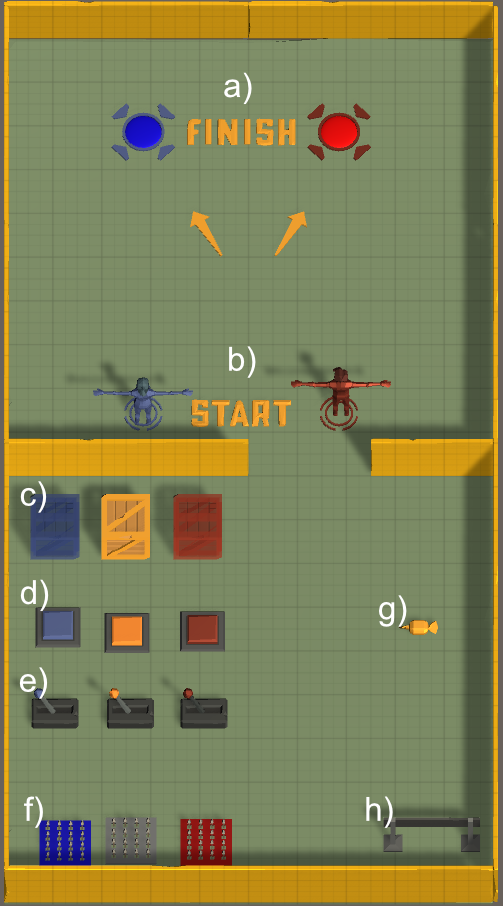
\includegraphics[scale=0.4]{images/lobby_game_elements.png}
    \caption{On this image all game elements for each level can be seen:
    a) goal points for each player b) start points and players c) movable boxes d) pressure plates e) switches f) traps g) candy h) barrier}
    \label{fig:game elements}
\end{figure}


Each level consists of a floor and walls. There are always two spawn-points, one for each player, as well as a goal-point for each player. The next level will load, as soon as both players are standing on their goal-point.


\begin{enumerate}
    \item Candy
    
    In each Level there are three candies players are able to collect. Each candy adds one score point to the shared team score.
    \item Movable box:   
    
    The movable box is blocking the way of the player. This box can be pulled towards the player or pushed in the forward direction of the player. It is not possible to move it side-wards, so the movements is limited to two direction, according to the player position.
    \item Barrier
    
    The barrier is blocking the players path like a box. The player itself is however not able to interact with it directly. A barrier can be disabled by other elements such as switches or pressure plates
    \item Switch
    
    A switch has the purpose of enabling or disabling objects. a switch can disable a barrier, so players can pass it.
    It is also possible to enable and disable traps with it.
    
    Some switches are connected together. Only when both switches are activated at the same time, they will stay active.
    \item Pressure Plate
    
    Pressure plates are similar to switches. However the difference to a switch is that it gets activated while a player is standing on top of it. It is also possible to move a box on top of it, so it will stay active while the both players can move around freely.
    
    There are also pressure plates that are connected with each other. Only while all connected pressure plates are active at the same time, a barrier for example is deactivated.
    \item Trap
    
    Each trap is sending the player back to the start, as soon as the player is standing on top of an active trap. An enabled trap has spikes, which disappear for a limited time. When the trap is disabled or the spikes are not visible, the player is able to move over the trap.
\end{enumerate}

The graphics for all listed elements can be seen in Figure \ref{fig:game elements}.

Movable boxes, switches, pressure plates and traps can also have the colour of one player. 
Blue pressure plates can only be activated while the blue player or a blue box is on top of it.
Blue switches can only be activated by the blue player and only the blue player is able to move a blue box.
Even if traps are coloured, both player will respawn when the collide with it.
The same is valid for the red player and red objects

To force the player to collaborate with their partner, a blue object can only be seen by the red player, and a red object can only the seen by the blue player. As both players are not able to see every object they can interact with, they need to tell their partner, where a object is, where a box needs to be moved to and which areas they need to leave untouched.

\subsubsection{Cooperative game mechanics}
\label{Cooperative game mechanics}

To give the players the possibility to interact with each other, there are following mechanics a player can use.

\begin{figure}[h!]
    \centering
    \begin{subfigure}[b]{0.4\linewidth}
        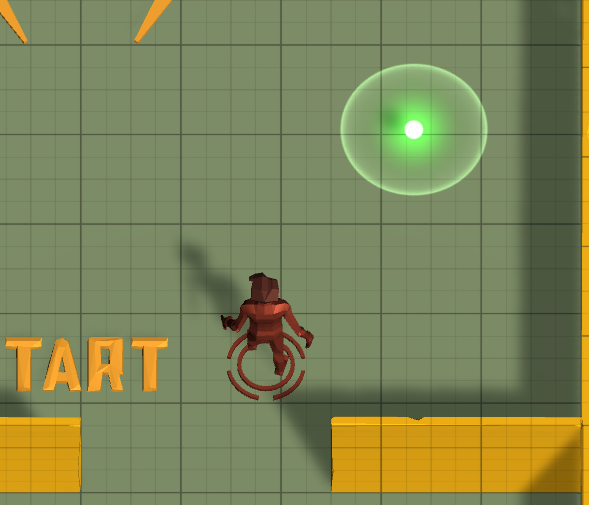
\includegraphics[width=\linewidth]{images/location_ping.png}
        \caption{Location ping}
        \label{fig:location ping}
      \end{subfigure}
    \begin{subfigure}[b]{0.4\linewidth}
        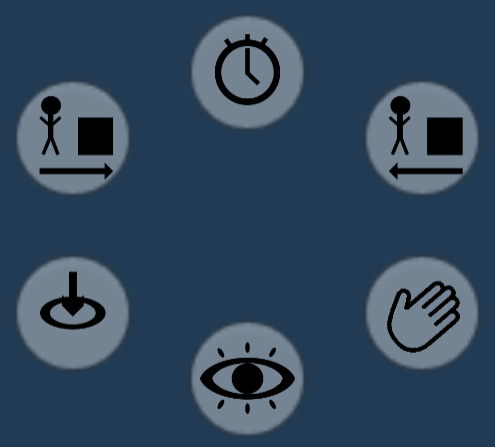
\includegraphics[width=\linewidth]{images/ping_types.png}
        \caption{All six ping types}
        \label{fig:ping types}
    \end{subfigure}
    \caption{ a) shows a placed location ping. 
    b) shows the selection user interface of all 6 advanced ping types players can use. By choosing the stopwatch-icon, a countdown at the selected position is placed. All other five options are placing icons for a temporary time onto the environment.}
\end{figure}

In the game are three types of pings available. As mentioned in
Section \ref{section:Attention-focusing}, pings are counted towards attention-focusing game mechanics. With a simple left click with the mouse, a location-ping is created at the clicked position. On figure \ref{fig:location ping} a location ping can be seen.
Besides a simple location-ping, a player can also use six semantically imbued pings. Figure \ref{fig:ping types} shows all six typed a player is able to choose. For time critical actions such as a time based switch, a countdown ping can be placed. The other 5 options should give the player the possibility to give commands to other players. 


\begin{figure}
    \centering
    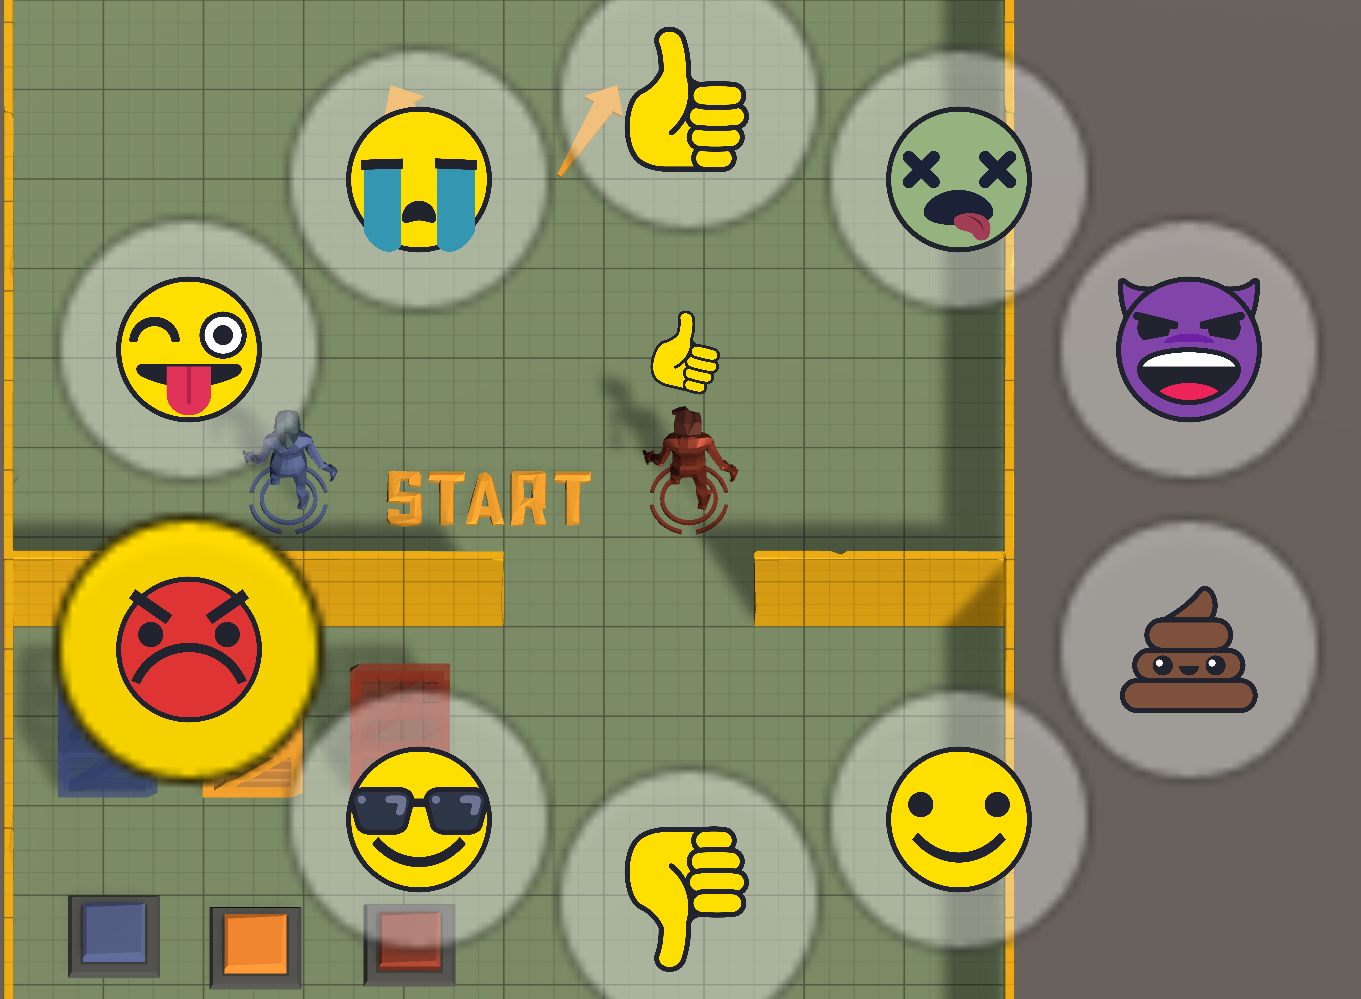
\includegraphics[width=0.5\textwidth]{images/emoji_selection.png}
    \caption{Selection interface of all emojis. Above player red, a thumbs-up emoji is displayed}
    \label{fig:emoji selection}
\end{figure}

For immersive communication, players get the option to use emojis.
Figure \ref{fig:emoji selection} shows all select-able emojis. The selection window opens while the right mouse button is pressed. The currently selected emoji is chosen when the right mouse button rises.
Besides all eight select-able emojis, an exclamation mark emoji is shown above the players head. The intention behind the emojis is to give the player a way to express their feelings. Players should have the possibility to describe their current emotional state without choosing wording. This communication mechanic is a expressive emotional game mechanic as described in \ref{section:Expressive}.


\begin{figure}
    \centering
    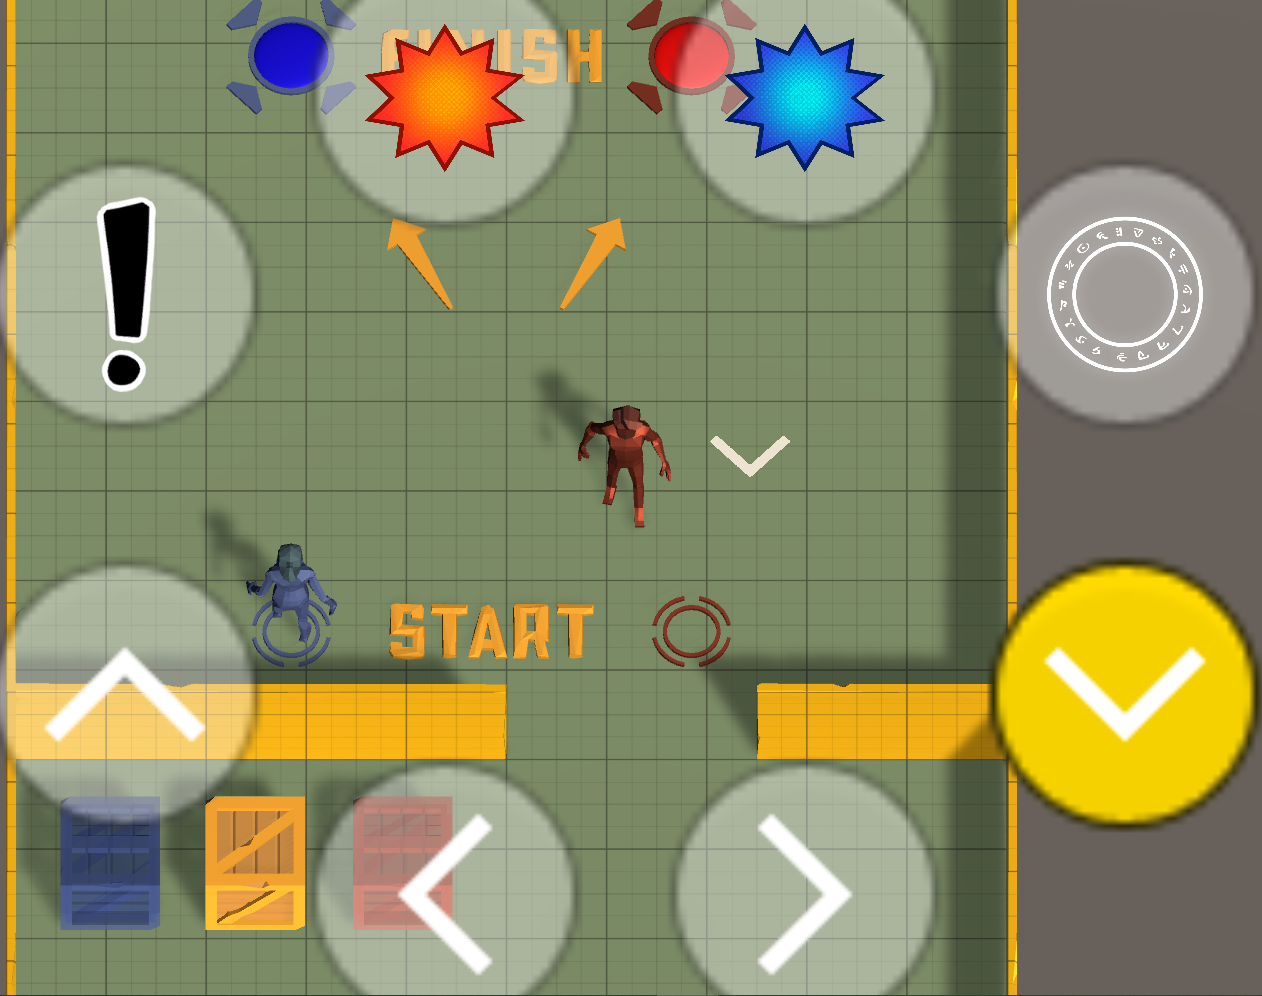
\includegraphics[width=0.5\textwidth]{images/decal_selection.png}
    \caption{Selection interface of all emojis. Above player red, a thumbs-up emoji is displayed}
    \label{fig:decal selection}
\end{figure}

To create longer lasting messages, players can create decals with 8 different images, seen in \ref{fig:decal selection}. This decal-system is an environment-modifying communication mechanic, described in \ref{section:Environment-modifying}. This images are placed onto the ground below the player. Every decal is overlapping the last one, but is not deleted. They last as long as the current level is player. With arrow marks on the floor as an example, players could mark a safe path which can be run along.


The fourth communication game mechanic is the recording of the current player position. While pressing the Ctrl-key or the middle mouse button, the current location of the player is saved. On release, a light transparent sphere with the player-colour is following the recorded path. This tool is not necessary a way to communicate with each other. It was implemented to test, if players would use the ghost for emergent cooperative communication as described in section \ref{section:Emergent}. Theoretically, it could also be used to "draw" signs by walking onto the environment. The main purpose however is, to give the user the possibility to record a save path they were able to run along.



\subsection{Gameplay implementations}
\label{section:Gameplay implementations}

character
    active player
    move
    interact
    Position Syncronisation
    Animation Syncronisation
    
camera

overlapping collider

move object

pressure plate

toggle

traps








\subsection{Implemented cooperative game mechanics}
\label{section:Implemented cooperative game mechanics}

Mechanics: 
\begin{itemize}
\item Record Ghost, 
\item Speechbubble with emotes/directions etc.
\begin{itemize}
\item kinda like message macros
\end{itemize}
\item location & augmented Environment Pings
\begin{itemize}
\item Portal 2 countdown-ping
\item special icon ping
\end{itemize}
\item Draw on screen with virtual cursor
\end{itemize}

Wie diese Implementiert wurden